% Search for all the places that say "PUT SOMETHING HERE".

\documentclass[11pt]{article}
\usepackage{amsmath,textcomp,amssymb,geometry,graphicx,enumerate,tikz}
\usetikzlibrary{arrows}
\geometry{a4paper}
\usepackage{mathtools}
\DeclarePairedDelimiter\ceil{\lceil}{\rceil}
\DeclarePairedDelimiter\floor{\lfloor}{\rfloor}

\def\Name{Nguyet Minh Duong}  % Your name
\def\SID{24444722}  % Your student ID number
\def\Login{N/A} % Your login (your class account, cs170-xy)
\def\Homework{7} % Number of Homework
\def\Session{Spring 2015}


\title{CS170--Fall 2015 --- Homework $\Homework$\textsl{•} Solutions}
\author{\Name, SID \SID}
\markboth{CS170--\Session\  Homework \Homework\ \Name}{CS170--\Session\ Homework \Homework\ \Name}
\pagestyle{myheadings}
\date{}

\newenvironment{qparts}{\begin{enumerate}[{(}a{)}]}{\end{enumerate}}
\def\endproofmark{$\Box$}
\newenvironment{proof}{\par{\bf Proof}:}{\endproofmark\smallskip}

\textheight=9in
\textwidth=6.5in
\topmargin=-.75in
\oddsidemargin=0.25in
\evensidemargin=0.25in


\begin{document}
\maketitle

Collaborators: Henry Kwan \& James Carlson

\section*{1. Name Distances}
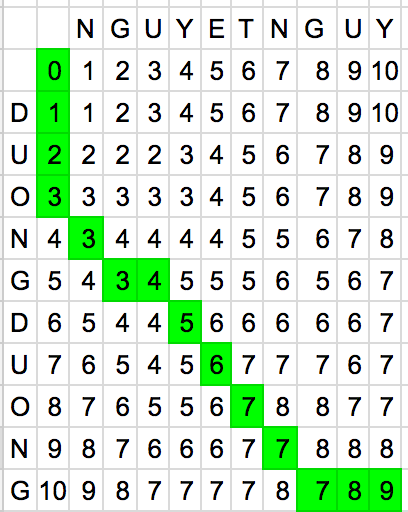
\includegraphics[scale=0.7]{hw71} \\

\newpage
\section*{2. Road Trip}
\begin{qparts}
\item[1.] Main Idea \\
Create an array, and make it such that all values less than 1 returns 0. We make iterate through the array indices, such that the value at a specific index, call this index $i$, is the minimum value of $(a_i + array[i - 1],(a_i + array[i - 2], ..., a_i + array[i - (k - 1)], a_i + array[i - k])$. After we finish the iteration through all N-values, we return the value at N. This is the minimum value of lodging cost. 
\item[2.] Pseduocode
\begin{verbatim}
Procedure MinLodgingCost(array: A, max travel distance: k):
  D := empty dictionary, where key is town, 
    and value is min distance to get there;
    for all keys less than, its value is 0. 
  last_town = size(A)
  
  for x from 1 to last_town:
    D[x] = A[x] + min(D[x-1], D[x-2], ..., D[x-k]
  
  return D[last_town]
    
\end{verbatim}
\item[3.] Proof of Correctness \\
At every single town, we checked for the lowest cost possible we can have given that we \textit{have} to sleep at that town for the night. For the first k-towns, it is whatever the rate is to sleep there. This is because we do not need to rest up until that point, so it is optimal for us to not rest at any town previous to it and just rest at that town. Which, in result, gives us the cost of the current trip to be whatever the rate is to sleep there for the night. However for all cities after k, looking back k-values and choosing the city with the lowest cost rate to get there (and sleep the night there) will give us the minimal cost of a trip to get to that point. Then we return the value of how much it costs at the last city, and we will get the minimal of the trip. 

\item[4.] Running Time Analysis \\
$O(nk)$ \\

For every single town, we store the value of how much it would cost to sleep there for the night into the dictionary. To go through the entire list of towns, it takes $O(n)$ times, n being how many towns there are. Then we look for k-towns backward to choose the town we can sleep at the night previous for the cheapest value (because we want to minimize the lodging cost), and add that cost to our cost of sleeping in this town tonight. To access the k-towns previous to the town we're at is $O(k)$. And since we have to do this for every single town we visit, we have to multiply the two running time $O(n) * O(k) \rightarrow O(nk)$
\end{qparts}

\newpage
\section*{3. Word Wrap}
\begin{qparts}
\item[1.] Main Idea \\
We will make a 2D array $A[x][y]$, such that x indicates the line we are on, and y indicates the number of words we have put inside of the line. $A[x][y]$ will give us the $s(x,y)$. In our case: $y = x + \frac{M}{2}$ and $x$ is the row we are on. We will start on row 1, and go all the way to row n because we know that at most there are n-lines. Then at the end, we will compare all the different number of trailing spaces we can have of the last line ($A[x]$) versus the number of possible trailing spaces we can ahve of the line $A[x-1]$. And how we determine this is using the equation given to us, which is $(A[x][i])^2 +( A[x-1][j])^{2}$, and we choose such an $i$ \& $j$ that will make the minimum of the previous equation. 

\item[2.] Pseudocode 
\begin{verbatim}
Procedure MinCost(num characters per word list: L):
  A[x][y] := an array that takes in two input:
    x, the row/sentence we are on
    y, the number of words we're putting into in
  for i in 1 ... n:
    for j in 1 ... M/2:
      A[i][j] = s(i, i+j-1) 
        // assume procedure s is what is described
        // in the problem
   start from 1 to n:
     record all possible data combination
     record all of data's begin and end
     record the cost of such instance
     run the next row of words based on recordings
   return minimum cost in record that ends on N
\end{verbatim}

\item[3.] Proof of Correctness \\
Every single line can have from one word up to $\frac{M}{2}$ words, where $\frac{M}{2}$ is the situation in which case that all the words in the line are single letter words. So it is logical to see that it can hold to at maximum that many words. So in the worst case scenerio, you check all $\frac{M}{2}$ words per line. In addition, in the worst case scenerio, is that every single word is its own line. \\

The next step is it figure out the best possible cost ending at N. I do this by iterating through the list of possibilities each one, and compare it to all of its previous possibilities, and record all of the values if we do a specific combination. Meaning, we try if $line_1$ ends with $word_3$, we test all the combination of $line_2$ such that it starts after $word_3$. We do this for all the iterations in $line_1$ and $line_2$, and repeat these steps all the way through $line_n$. \\

Now that we have recorded all the different possibilities manually, and it's ending position for that specific cost. We can iterate through the record, and pull out the smallest value of cost that ends on the $word_n$. That should give us the smallest cost. 

\item[4.] Running Time Analysis \\
$O(n)$

For the first iteration, we go through all the $\frac{M}{2}$ values, for every single word, which is $n$. This gives us the run time of $O(\frac{M}{2} * n)$ to do all of the calculations and inputting the values. Then for the second iteration, we look at all of the possible combination of values for every single possible line. What this means is we did $n$ lines, and in every single line we looked through all the combination possibility, which is $(\frac{M}{2})^2$. Then we have to look through all the possibility combination and see which one gives us the best value. This is $O(n\frac{M}{2})$, because every single one stores that many different possibilities because it compares to its pair. \\

This gives the run time of $O(n(\frac{M}{2})^2 + n\frac{M}{2} + (n\frac{M}{2})$. However because $M$ is a constant, we can remove it in our run time. So now it is $O(3n)$. Since 2 is also a constant, our run time is $O(n)$. 
\end{qparts}


\newpage
\section*{4. Pebbling a Checkerboard}
\begin{qparts}
\item 8 different patterns. \\

The following are the different patterns it can take, where 0 means\\
 empty and 1 means it has a pebble: \\
$[0 0 0 0$] \\
$[1 0 0 0]$ \\
$[0 1 0 0]$ \\
$[0 0 1 0]$ \\
$[0 0 0 1]$ \\
$[1 0 0 1]$ \\
$[1 0 1 0]$ \\
$[0 1 0 1]$

\item \begin{qparts} \item[1.] Main Idea \\
We start our search for the best pattern and cost on the second one. We record all the different combination that are compatible of the $column_1$ and $column_2$. And for each possible combination, we record the cost along with what type of $column_2$ is. Then we compare $column_3$ with $column_2$ in the same manner, taking in consideration of what types $column_2$ can be and all of the compatible types of $column_3$ and record all of the costs there. Continue until we reach $column_n$, in which case at the end, we just return the recording of how much the costs of each type of variations are. Return the biggest cost from $column_n$, and tracks which columns were used to build it. We know it is valid because we built it from the left. 
\item[2.] Pseudocode
\begin{verbatim}
Procedure OptPlace(A[c]):
  // A[c] returns the columns
  types(A[1]) <- all 8 types 
    // types records what types is valid
    // for a specific column
  for i in 2 ... sizeOf(A):
    for all i types(A[i-1]):
      for all types T of A[i]:
        if isCompatible(i, T): 
          // lets us know if the two are legal placements
          A[i].cost(T) = A[i-1].cost(t) + A[i].cost(T)
          // cost returns the cost of that specific placement
          types(A[i]).include(T)
          prev(A[i].cost(T)) = i // records the previous column's pattern
  T := max(A[n].cost(type1), A[n].cost(type2), ..., A[n].cost(type8))
  G[] := array that tells us which types we need to build to get max cost
  G[sizeOf(A)] = T   
  for i in sizeOf(A) - 1 ... 1:
    G[i] = prev(A[i+1].cost(G[[i+1])))
  return G
\end{verbatim}
\item[3.] Proof of Correctness \\
\textbf{Proof by Induction}, induct on n the number of columns \\
For the first column, its best value is just whatever value gives us the most "cost," and it is in relation to a specific type. So when we compare the next one to it, we need to take in consideration of type compatibility, where the column next to it must be compatible to the one previous to it, and the new cost of the column will also give us the previous. Assume this works up to k columns. For k+1 column, then, we only need to take in consideration of its previous and whether or not it is compatible. Then to compatible ones, we should add up all the total cost if we end up having that specific type. In the end result, it gives us all of the possible types, and how much costs we would have if we were to use it. 
\item[4.] Running Time Analysis \\
$O(n)$ \\

We know that there are 8 different types. So in our algorithm, our first loop, we find every single combination between its current value and the previous. That means we iterate through n values, and do 64 different comparison and recording on it. This gives us the run time of $O(64n)$. Then at the end, we iterate through all of the previous, and we know that we have the size of the previous is at most n. Therefore this is a $O(n)$ path search. The combination of the two is $O(65n)$ but constants are removed so it is just $O(n)$. 
\end{qparts}

\end{qparts}

\newpage
\section*{5. Treeland Tourist}
\begin{qparts}
\item[1.] Main Idea \\
Start at the node without any children. Start with the base case of this situation. So we record how many cities it can traverse in this case (one), and what is the cost (zero). The point is to record the minimum cost it requires to travel 1 ... k cities, and have all of those costs stored in the node. Then when we reach the parent node, we choose either the children with the least cost to travel those specific number of nodes, or the combination of the children's smaller travel amounts to see the minimum cost we'd need to travel k amount of cities. By the time this algorithm ends, we should be able to ask the root node for the minimum cost if we travel k nodes. 
\item[2.] Pseudocode 
\begin{verbatim}
Procedure LeastPaths(Graph G, k):
  Q := empty queue
  for all nodes N without children:
    N[1] = 0 // store the value of how much it cost
      // to traverse i (in this case 1) city at this node
    Q.push(N) // pushes node N to the end of the queue
  while Q is not empty:
    N = Q.pop() // removes the first item of the queue
    P = N.parent() // returns the parent of node N
    P[1] = 0
    for i in 1 ... k:
      for j in 0 ... i:
        if P[i+j] > N[i] + cost(N,P): // assume if P[x] DNE -> inf
          P[i+j] = N[i] + cost(N,P)
     P.push()
  R = root(G) 
  return R[k]
\end{verbatim}
\item[3.] Proof of Correctness \\
\textbf{Proof by Induction}, on n the number of vertices. \\
The base case for this problem are the nodes without any children. In this case, there is only one node we can traverse. It is this node, and the cost to travel is zero because we cannot go anywhere. Assume this works for all parents nodes up to and including K. Then for the parent of this K's node, call it P, we need to take in consideration all the possibiltiies, and its minimum cost. The possibilities are if we don't traverse P's children. Then in which case, we look at the previous base case. Otherwise, we do traverse P's children, and find all the possibilities of the traversal in the most minimalistic way. To do this, we compare the cost travel 2 to k nodes from both the left and right child. In addition to this, we need to find all the possible combination to add up the values from 2 to k, using both the right and left child minimum cost to travel. Hence it will also return the minimal value at the node, for a specific k number of nodes needed to traverse. \\

So if we run this algorithm and complete it, the root node should have the all the minimal cost to traverse all numbers of cities from 1 to k cities. As a result, we can call on the kth city, and have it return the value. 

\item[4.] Running Time Analysis \\
$O(nk^{2})$ \\

We look through all nodes. This is a run time of $O(n)$. However within each node, we look for all the different combinations to figure out the minimum cost for traveling a 1 ... k cities. This means that for every single number of cities we want to check k cities, and the k different combinations we could make. So for each node, there is actually $k^2$ searches, which gives us $O(k^2)$ running time to do a specific task. A combination between these two will give us $O(nk^2)$. 
\end{qparts}

\newpage
\section*{6. Sponsored Search Auctions}
TBH I figured out part A, but I am going to hackingEDU so no time to type it up. Only because I have an essay due in thirty miutes though. Please spare me :(
\end{document}
